
\chapter{Introducci\'on}
\label{ch:Introduccion}

\section{Estado del arte}

En este punto comenzaremos estudiando algunos dispositivos existentes en la actualidad y que son utilizados para la monitorización del cuerpo humano así como las prestaciones de cada uno de ellos.

Posteriormente se realizará un sondeo de los métodos y procedimientos adoptados en diferentes estudios para el análisis de los ajustes posturales anticipatorios en diferentes casos, así como las aplicaciones de los mismos.

Finalmente, hablaremos de las técnicas más comunes de calibración, preprocesado y clasificación.

\subsection{Instrumentaci\'on}

Existen varios tipos de dispositivos usados para la medida de los APAs, destacando: el electromiógrafo, las plataformas de fuerza, los sensores inerciales y dispositivos basados en cámaras.

La electromiografía (EMG) es una técnica que nos da información sobre la actividad eléctrica de los músculos del esqueleto (Ver figura [1]). El electromiógrafo es capaz de detectar la actividad eléctrica debido a una diferencia de potencial en las células musculares, siendo muy útil, además de para el análisis de posturas corporales,  para localizar lesiones como parálisis musculares y el lugar donde éstas se producen \cite{Marcio2010} \cite{Instr1}. 


Hasta el momento, la gran mayoría de los estudios realizados han incluido como dispositivo de medida, entre otros,  una plataforma sensible a la fuerza y la presión.  Sin embargo, el coste y la complejidad de medir los APAs con un análisis del movimiento tradicional, usando plataformas de fuerza y sistemas EMG limita sus aplicaciones en la práctica clínica. Por ello, recientemente se ha optado por sensores inerciales pequeños, baratos y portables. Aun así, en nuestro caso, se ha utilizado dicha plataforma, contemplando la posibilidad de prescindir de ella en un futuro \cite{Mancini2009} \cite{Vennila2011}.

Los dispositivos fundamentados en sensores inerciales comúnmente utilizados son las IMU (inertial measurement unit) , un dispositivo electrónico que mide e informa acerca de la velocidad, orientación y fuerzas gravitacionales de un aparato, usando una combinación de acelerómetros y giróscopos.
 También existe la posibilidad de combinarlos con magnetrómetros, pasándose a llamar MIMO. Algunos de los dispositivos MIMO existentes actualmente en el mercado son: 3DN-GX4-45 \cite{Instr2},  xsens-mvn \cite{Instr3} y mvn-biomech \cite{Instr4}, donde todos ellos utilizan sensores de tipo Microelectromecánico (MEMS).
 
 \begin{figure}[H]
 	\centering
 	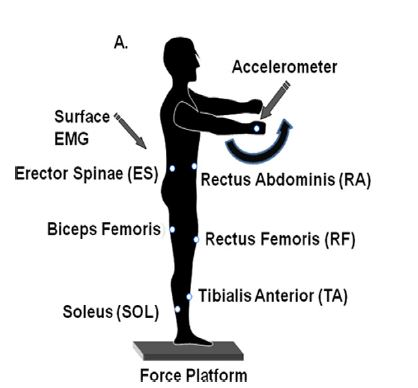
\epsfig{file=imagenes/Captura, width=7cm}
 	\caption{EMG, acelerómetros y plataforma \cite{Gay2011}.}
 	\label{fig:arte1}
 \end{figure}
 
Existen marcadores de reflexión infrarroja que nos da una medida más compleja de la postura. Estos se reparten por el cuerpo y nos pueden proporcionar información sobre estrategias posturales, lo que nos permite saber si el balanceo del cuerpo se realiza teniendo como punto central de oscilación el tobillo o se debe movimiento de cadera, por ejemplo . En la figura [2]se muestra la disposición del sistema.

\begin{figure}[H]
	\centering
	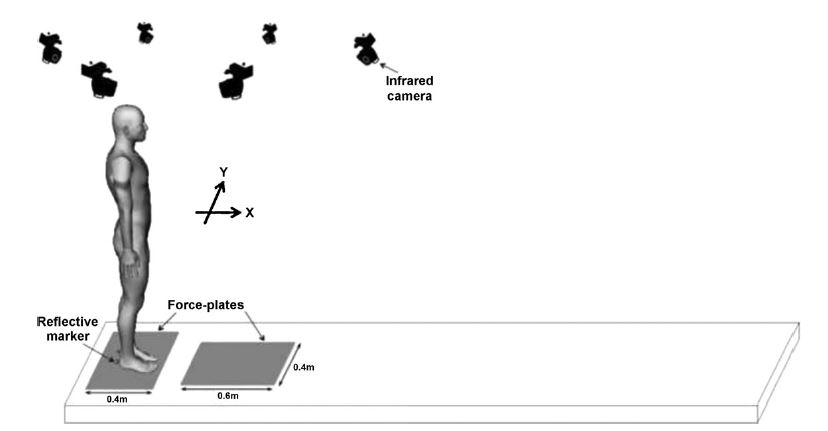
\epsfig{file=imagenes/Captura2, width=7cm}
	\caption{Esquema con mascadores de reflexión infrarroja \cite{Teddy2013}.}
	\label{fig:arte2}
\end{figure}

Como se ha mencionado anteriormente, también existe la posibilidad de utilizar sensores basados en cámaras que generalmente forman parte de sistemas ópticos de captura del movimiento humano, tales como Kinect \cite{Instr5}.


\subsection{M\'etodos y procedimientos}

Hasta el momento se ha realizado numerosos estudios acerca de los Ajustes Posturales Anticipatorios, principalmente en los últimos seis años. 
La finalidad de la mayoría de estas investigaciones es poder profundizar en el conocimiento de qué es lo que realmente ocurre cuando iniciamos un determinado movimiento, si este hecho sigue un determinado patrón y de las condiciones de las que depende.

Si analizamos el estado del arte de los APAs podemos encontrar que las primeras investigaciones intentaban confirmar la hipótesis de si los APAs estaban asociados a un movimiento voluntarios, confirmándose así la hipótesis y llegando a la conclusión de que es más probable que los ajustes no aparezcan cuando el inicio el movimiento no está planeado, es decir, cuando es evocado por una perturbación. Esto es esencial en el control del balance en el momento de andar ya que el conocimiento de esto se podría utilizar para prevenir caídas en personas con dificultades de movilidad, por ejemplo.\cite{Mcllroy1993}\cite{Yiou2012}\cite{Teddy2013}\cite{Bouisset2008}\cite{Neeta2014}

Posteriormente se han ido comprobando la influencia de otro tipo de variables, como la realización de ejercicios diversos donde se estimulan músculos diferentes y la reacción de dichos músculos\cite{Gay2011}; la influencia de la edad para generar patrones posturales \cite{Bleuse2006} \cite{Estelle2008}; el tipo de señal que inicia el movimiento (visual o auditiva) ya que influye en la reacción del cuerpo ante dicha estimulación \cite{Mcllroy1993}\cite{Antonia2009}\cite{Vicent1999}\cite{Tard2013}; como el miedo a caerse afecta a la postura que se adopta al iniciar a andar[26] o como enfermedades neurodegenerativas, como Parkinson o la Esclerosis múltiple\cite{Mancini2009}\cite{Jebb2008}\cite{Chris2005}\cite{Hall2013}, o parálisis cerebrales, tales como hemiplegia o diplegia\cite{Hall2013}, generan diferencias en los APAs.

Todos estos estudios tienen una gran importancia en aplicaciones médicas. Por ejemplo, tal y como se ha dicho anteriormente, hay enfermedades que afectan al sistema nervioso central y por tanto, a la movilidad, provocando en muchas ocasiones caídas lo que implica que estas personas que las sufren padezcan miedo a volver a caer de nuevo. El hecho de confirmar que el propio miedo a la caída provoca variaciones en los APAs haciendo que estas personas sean más propensas a nuevas caídas nos podría ayudar a prevenirlas.

\subsection{An\'alisis de datos}

En los últimos años se han realizado numerosos trabajos relacionados con la calibración de acelerómetros y giróscopos, aunque la mayoría muestran pequeñas variaciones con respecto a otros estudios realizados anteriormente. Uno de los trabajos más destacados \cite{Kian2011}muestra una forma de realizar la calibración colocando los acelerómetros en seis posiciones diferentes y aplicando algoritmos algebraicos sencillos a los datos obtenidos. El giróscopo de calibra de forma distinta, mediante una proceso basado en una rotación conocida. A parte de este método anterior, existen otros basado al igual que él en la colocación de los acelerómetros en seis posiciones.

Existen otros métodos que intentan ser más precisos, aumentando el número de posiciones en las que se realiza la recogida de datos \cite{Camps2009}. También existen otro tipo de técnicas de calibración como algoritmos basados en operaciones algebraicas básicas o basados en filtros FIR. \cite{A.Olivares2013}

En cuanto a la estimación de la orientación para la monotorización del cuerpo humano, si se realiza un estudio de los trabajos existentes hasta el momento se puede ver que casi todos ellos se basan en la utilización del filtro de Kalman, sin embargo el resultado con señales de baja intensidad no suele ser muy preciso.\cite{A.Olivares2013}

Finalmente, analizamos el estado del arte del reconocimiento de movimientos en humanos y clasificadores. Rápidamente se puede ver que la cantidad de información relativa al campo de la clasificación en bastante grande, existiendo numerosos artículos y libros con información acerca de ello. Sin embargo, existen otro tipo de estudios, como en el que nos centraremos \cite{Banos2012}, donde se exponen métodos para el reconocimiento de actividad humana basados en un clasificador jerárquico ponderado. En él se indican diferentes esquemas de clasificación que podrían ser usados y que mejores resultados proporcionan para reconocer secuencias de actividad, tales como andar o correr.

